\graphicspath{{chapters/12/images}}
\chapter{Toward defining the course of evolution: minimum change for a specific tree topology}
“It has been a goal of those attempting to deduce phylogenetic relationshps on biological characteristics to find the ancestral relationship(s) that would permit one to account for the descent of those characteristics in a manner requiring a minimum number of evolutionary steps or changes.
The result could be called the most parsimonious evolutionary tree and might be expected to have a high degree of correspondence to the true phylogeny (Camin and Sokal, 1965)”

\section{Maximum parsimony principle}
Two definition of the \textbf{maximum parsimony principle} are:
\begin{itemize}
\item ”find the ancestral relationship(s) that would permit one to account for the descent of those characteristics in a manner requiring a minimum number of evolutionary steps or changes" (Fitch)
\item ”We believe that selection was more likely to discover the utility of a
mutation in two closely related, and possibly contemporaneous, lines of
descent than that a mutation once found beneficial should then become
deleterious relative to its previous ancestral form”
\end{itemize}

They arise from Occam’s razor and minimum description length principle. However, we might find mutations that are neither beneficial nor detrimental.
\\
from entry “Simplicity” on Stanford’s Philosophy Enciclopedia:
“Most philosophers believe that, other things being equal, simpler theories are better. But what exactly does theoretical simplicity amount to? Syntactic simplicity, or elegance, measures the number and conciseness of the theory's basic principles. Ontological simplicity, or parsimony, measures the number of kinds of entities postulated by the theory."

\subsection{Maximum parsimony method}
The most parsimonious (phylogenetic) tree is the one with lowest score, where the score is the number of mutations. An example is shown in figure \ref{fig:intro}.

\begin{figure}[H]
		\centering
		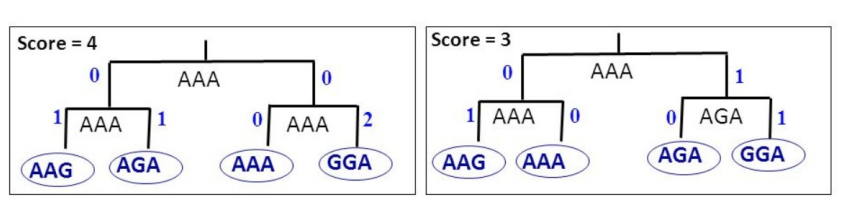
\includegraphics[width=0.9\textwidth]{1.png}
		\caption{Most parsimonious tree is the one on the right, because it has a lower score. }
		\label{fig:intro}
	\end{figure}

\section{Introduction}
The justification of finding the a most parsimonious tree lies in the most efficient use of the information available and does not presuppose that evolution follows a most parsimonious course. The numerical taxonomic procedure seen in the chapter before (Fitch and Margoliash, 1967) provide dendograms that could be among the more parsimonious solutions, but there's no way to be sure.
\\
A sub-problem to finding the most parsimonious tree(s) is finding all possible, most parsimonious assignments of the information to any given particular tree. The solution provides the most reasonable hypotheses on the ancestral states and therefore is the best estimate of the course of evolution.
The biological characteristics to be used are the nucleotides of ortologous genes (but the method is applicable to any data for which the underlying assumptions are acceptable).
\\
Given a set of descendent nucleotide sequences and a topology presumed to describe their ancestral relationship one cans et forth:

\begin{itemize}
\item The minimum number of mutations to account for the descent of those sequences from a common ancestor;
\item all possible ancestral sequences at each node (branching point);
\item combinations of nodal ancestral sequences;
\item a way of assigning relative weights among the various alternative nucleotide replacements.
\end{itemize}

\section{Method}
Task: given a tree whose topology has been already determined find for each taxonomic unit its ancestral value at each node, following the maximum parsimony principles.
\subsection{Assumptions}
The assumptions are:
\begin{itemize}
\item A set of ortologous descendant sequences is available;
\item the ancestral relationships among them are known;
\item any nucleotide may replace any other other nucleotide at any position. The word \textit{may} indicates that all logical options are to be considered, not denying however the possibility that selective forces may have an impact on some options.
\end{itemize}

Each position can have as a value the nucleotides A, C, G, or U or some combination of the,. Ambiguity can arise because of uncertainty of the codon (redundancy of the genetic code), or uncertainty about ancestral character states. An unknown position is represented by a set of letters.
\\
The algorithm must be repeated for every nucleotide position in the gene. The reconstruction of the ancestral gene the follows two phases, the preliminary phase, in which nucleotides are placed on all ancestral nodes, and a final phase in which corrections to the preliminary assignments are made.
Finally, since not every possible link should be treated as equally representative of those events that did occur in the descent, "probabilities" are assigned to each link.


\subsection{Reconstruction of possible ancestral nucleotides-preliminary phase}
\begin{figure}[H]
		\centering
		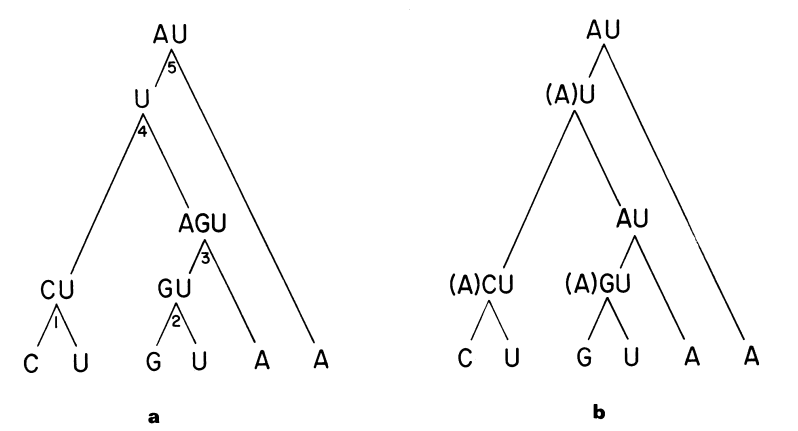
\includegraphics[width=0.9\textwidth]{2.png}
		\caption{Reconstruction of ancestral nucleotide forms }
		\label{fig:preliminary}
	\end{figure}

The preliminary phase proceeds from the descendent character sets by formulating an ancestral character set for an immediate ancestor and working backward, one successive node at a time, until the nodal character set for the most distant ancestor has been formed.
The formulation of each nodal set follows the simple rule: The preliminary nodal set shall be comprised of all characters (nucleotides) common to both immediately descendent sets; if none are common to both, then the preliminary nodal set will be comprised of all characters found in either.
In mathematical terms, the nodal set is the intersection of its immediately descendant sets if the intersection exists (i.e., is not empty) otherwise it is the union of those sets. An example is shown in figure \ref{fig:preliminary}a (on the left).
\\
Following the example in figure \ref{fig:preliminary}a: because there are so many different nucleotides in only 6 taxonomic units, many of the descendants have no nucleotides in common, with the result that the first (lowest) three preliminary nodal sets are formed by unions. At the penultimate node [4], the intersection $CU \cap AGU = U$ and so U is the preliminary nodal set. The ultimate node is once again a union. Note that with real amino acid sequences such as the cytochromes \textit{c}, the vast majority of the nodal sets are simpler in that they are formed by intersections of identical elements.
\\
It should be noted that for every occasion that a union is required to form the preliminary nodal set, a mutation (nucleotide replacement) must have been fixed in this nucleotide position at some point during the evolution of this position.

\subsection{Reconstruction of possible ancestral nucleotides-final phase}
The necessity of a second phase arises from the deficiencies of the preliminary phase.

\begin{figure}[H]
		\centering
		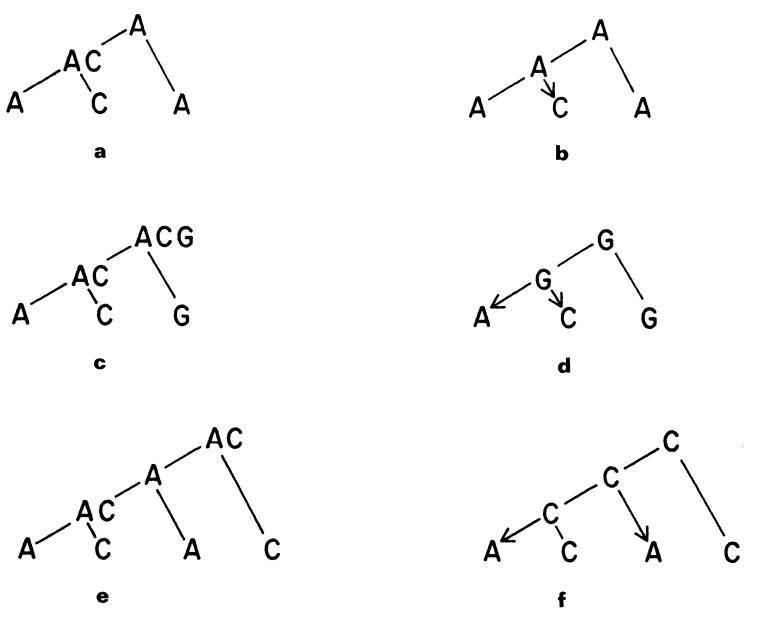
\includegraphics[width=0.9\textwidth]{3.png}
		\caption{Deficiencies of preliminary phase reconstruction. }
		\label{fig:deficiencies}
	\end{figure}

IN figure \ref{fig:deficiencies}a the ambiguous AC represents an initial inability to decide whether the ancestral form was an A replaced by a C or vice versa. The only certainty is that one replacement is required. The only formulation that will permit the descendent positions to be accounted for in a single replacement requires that replacement from A to C. The elimination of C from the first node is determined by the \textit{rule of diminished ambiguity}. The rule is described in steps I and II of the algorithm.
\\
Figure \ref{fig:deficiencies}d shows an equally adequate solution to that of \ref{fig:deficiencies}c. The fact that G is an valid alternative for the first node in encompassed by the \textit{rule of expanded ambiguity}, which is described in steps III and IV.
\\
In Figure 2e (lower left) is shown a third preliminary phase reconstruction that accounts for four descendants using two replacements. Figure \ref{fig:deficiencies}f is a valid alternative. Indeed, the C at the lowest node is a valid alternative to A if and only if a C is allowed at the penultimate node above. Two nodes contain a nucleotide not present in the intervening node because of the intersection process. Hence this is called the \textit{rule of encompassing ambiguity}, described in step V.

\subsubsection{The algorithm}
\begin{itemize}
\item \textbf{I}: If the preliminary nodal set contains all of the nucleotides present in the final nodal set of its immediate ancestor, go to II, otherwise go to III.
\item \textbf{II}: Eliminate all nucleotides from the preliminary nodal set that are not present in the final nodal set of its immediate ancestor and go to VI.
\item  \textbf{III}: If the preliminary nodal sey was formed by a union of its descendant sets go to IV, otherwise V.
\item \textbf{IV}: Add to the preliminary nodal set any nucleotides in the final set of its immediate ancestor that are not present in the preliminary nodal set and go to solution which is not encompassed by the VI.
\item \textbf{V}: Add to the preliminary nodal set any nucleotides not already present provided that they are present in both the final set of the immediate ancestor and in at least one of the two immediately descendent preliminary sets and go to VI.
\item \textbf{VI}: The preliminary nodal set being examined is now final. Descend one node as long as any preliminary nodal sets remain and return to I above.
\end{itemize}

Figure \ref{fig:intro} shows the operation of the algorithm.

\subsection{Permitted links between nucleotides in successive nodal sets}
Figure \ref{fig:temporal} is a redrawing of the ancestral nodes of figure \ref{fig:intro}b with links connecting those nucleotides that comprise valid lines of descent in a most parsimonious tree. The arrowheads are on the internodal links that involve a change of nucleotide.

\begin{figure}[H]
		\centering
		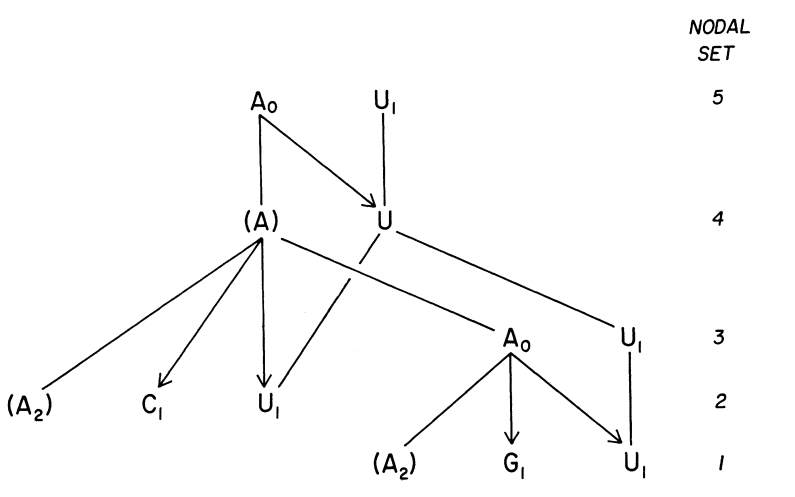
\includegraphics[width=0.9\textwidth]{4.png}
		\caption{Possible temporal sequence of ancestral nucleotides. }
		\label{fig:temporal}
	\end{figure}

The subscripts give the number of nucleotide replacements required in those cases where
one or both immediate descendants are not other ancestral nodes. Since node 4 has only other ancestral nodes for its immediate descendants, its nucleotides have no subscripts.
\\
In figure \ref{fig:temporal} a complete phylogeny will require a network composed of one nucleotide from every node using only the links shown. Such a complete linkage will involve nucleotides with subscripts and possibly links bearing arrowheads. The sum of the arrowheads plus subscripts on any complete valid linkage is 4, the minimum number of replacements required to account for the data.
\\
How does one discover all the possible linkages like in figure \ref{fig:temporal}?
First, the nucleotides without parentheses were placed in the nodal set during the preliminary phase, while those with parenthesis during the final phase. Such nucleotides will be represented as $N_i$ and $(N_i)$, where the subscript denotes one of the four nucleotides.
An arrow is used to denote descent from an ancestor tot he next node.  Thus $(N_i) \rightarrow N_j$ means that an ancestral nucleotide that was added to a nodal set during the final phase of reconstruction is replaced (since $i \neq j$) by a nucleotide that was originally assigned to the descendant nodal set in the preliminary phase. An example is $(A) \rightarrow (C)$ in figure \ref{fig:temporal}.
\\
The rules are then as follows: given that a particular ancestral nucleotide is i,
\begin{itemize}
\item \textbf{I}: $N_i \rightarrow N_i$ or $(N_i) \rightarrow N_i$ is obligatory i f the descendent $N_i$ exists, if it does not, then:
\item \textbf{II}: all possible linkages are permitted except $N_i \rightarrow (N_j)$ and $(N_i) \rightarrow (N_j)$
\end{itemize}

\subsection{"Probabilities associated with specific links}
The number of fixations (back mutation) ascribed to a single nucleotide position is the same for all of the most parsimonious tree, it should be clear from figure \ref{fig:temporal} that which nucleotide replaces which is a function of the particular set of valid linkages that is examined. What then is the best estimate of the weight that should be assigned to any given link in the most parsimonious tree for the time period represent?
\\
A caveat is necessary. In real world descendent sequences, there will be events for which there's no evidence (i.e. we compute the event $A \rightarrow G$, but it really went like $A \rightarrow C \rightarrow G$). The weighting procedure only accounts for evident events and the "probabilities" obtained sum up to 1. However, since the real world is less parsimonious than the more restricted computational world, every such probability necessarily overestimates the likelihood that that event actually occurred in the evolutionary history of that nucleotide position, hence the quotation marks. This  computation is pursued anyway, since for most purposes we do not need to know the likelihood of events for which there is no evidence.

\subsubsection{The procedure for calculating "probabilities"}

\begin{figure}[H]
		\centering
		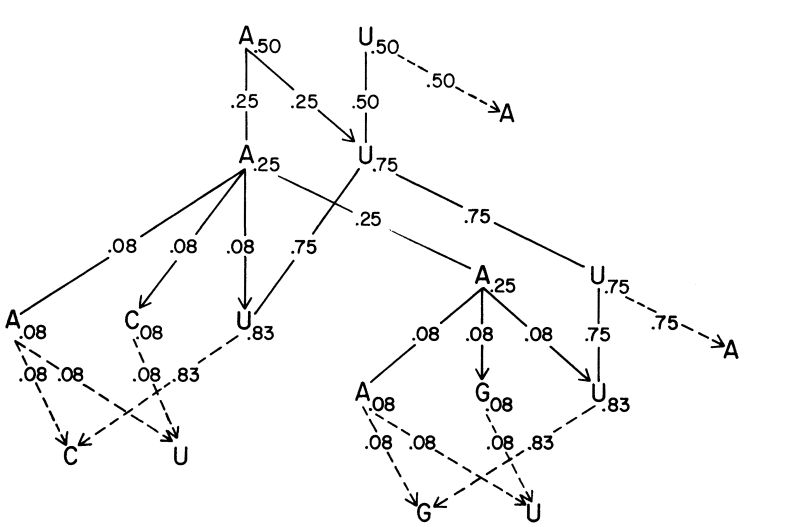
\includegraphics[width=0.9\textwidth]{5.png}
		\caption{"Probability" that segments are part of the temporal sequence of descent.}
		\label{fig:prob}
	\end{figure}

Assumption: all permitted nucleotides for the ultimate ancestor are equiprobable (i.e., in figure \ref{fig:prob} $P(^5 A) = P(^5 U) = 0.5)$.
This is to tackle the bias in favor of the predominating nucleotide in the line descending from the ultimate ancestor that has the fewest bifurcations. This bias comes from the assumption that all possible valid sets of complete linkages are equiprobable.
\\
Our assumption also assumes that every valid link from a given nodal nucleotide, $L(^k N)$, is equiprobable. Thus, the probability that a link is correct is $P[L(^k N)] = P(^k N) / n$, where $n$ is the number of links descending from $^k N$.
\\
In figure \ref{fig:prob} the dotted lines are the probabilities associated with every link and every nodal nucleotide shown in figure \ref{fig:temporal}.

\paragraph{Notes}
	If you want to have a look at the algorithm step by step, take a look at the slides of lecture 14.
